 \centering

     \begin{subfigure}[b]{0.3\textwidth}
        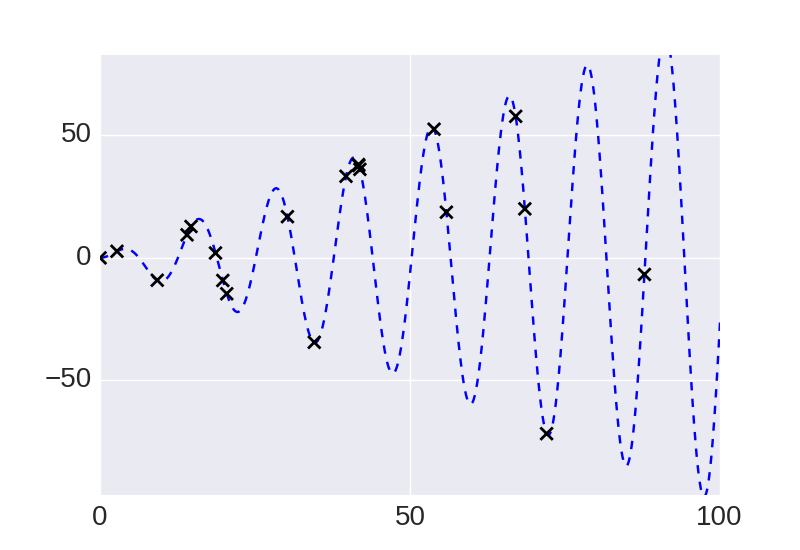
\includegraphics[width=\textwidth]{figs/composition/composition_demo_raw_data.png}
        \caption{Raw Data}
    \end{subfigure}
    ~ %add desired spacing between images, e. g. ~, \quad, \qquad, \hfill etc. 
      %(or a blank line to force the subfigure onto a new line)
    \begin{subfigure}[b]{0.55\textwidth}
\small
     \begin{align*}
        \klin &=   \sigma_1^2(x x^\prime)\\
    \kper &=  \sigma_2^2 \exp \bigg( \frac{2 \sin^2 ( \pi (x -
x^\prime)/p}{\ell^2} \bigg)\\ 
    \klin \times \kper &=  \sigma_1^2(x x^\prime)\, \sigma_2^2 \exp \bigg( \frac{2 \sin^2 ( \pi (x - x^\prime)/p}{\ell^2} \bigg) 
    \end{align*}\vspace{0mm} 
        \caption{Kernels}
    \end{subfigure}\vspace{4mm} 




Prior predictive, $\ybf_* \sim \mathcal{N}\big(0,K(\xbf_*,\xbf_* \midtheta)\big)$:

     \begin{subfigure}[b]{0.3\textwidth}
        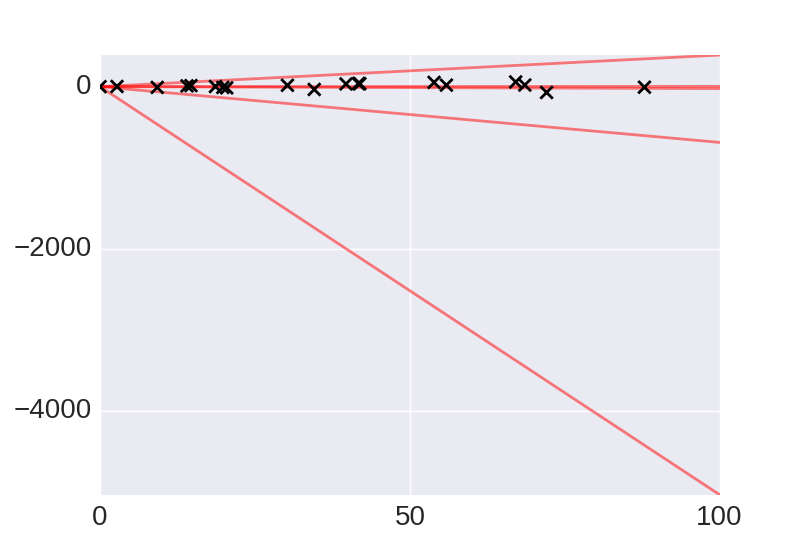
\includegraphics[width=\textwidth]{figs/composition/composition_demo_LIN_prior.png}
        \caption{$\Klin$}
    \end{subfigure}
    ~ %add desired spacing between images, e. g. ~, \quad, \qquad, \hfill etc. 
      %(or a blank line to force the subfigure onto a new line)
    \begin{subfigure}[b]{0.3\textwidth}
        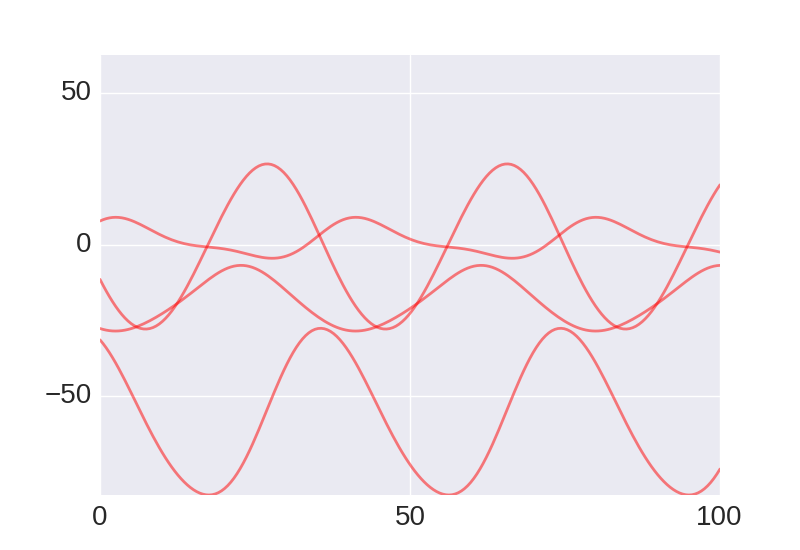
\includegraphics[width=\textwidth]{figs/composition/composition_demo_PER_prior.png}
        \caption{$\Kper$}
    \end{subfigure}
    ~ %add desired spacing between images, e. g. ~, \quad, \qquad, \hfill etc. 
    %(or a blank line to force the subfigure onto a new line)
    \begin{subfigure}[b]{0.3\textwidth}
        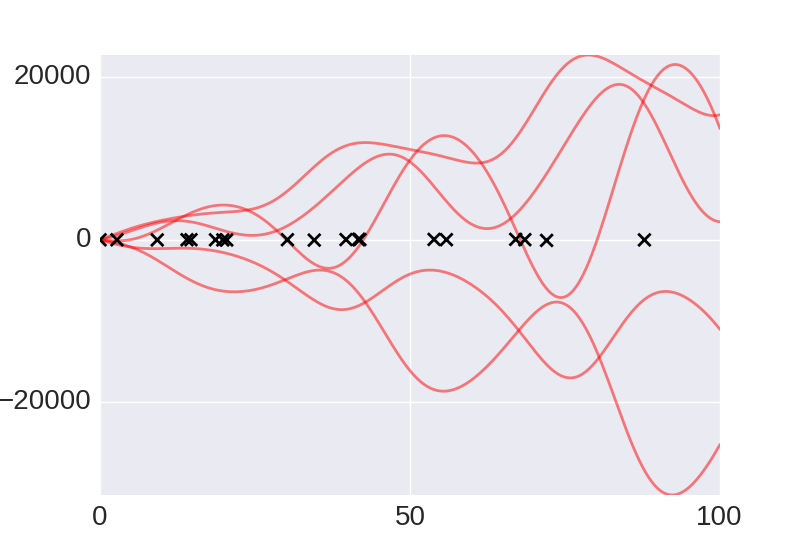
\includegraphics[width=\textwidth]{figs/composition/composition_demo_LINxPER_prior.png}
        \caption{$\Klin \times \Kper$}
    \end{subfigure} \vspace{4mm} 

Posterior predictive $\yprime \sim \mathcal{N}(\mupost,\Kpost)$:

 \begin{subfigure}[b]{0.3\textwidth}
        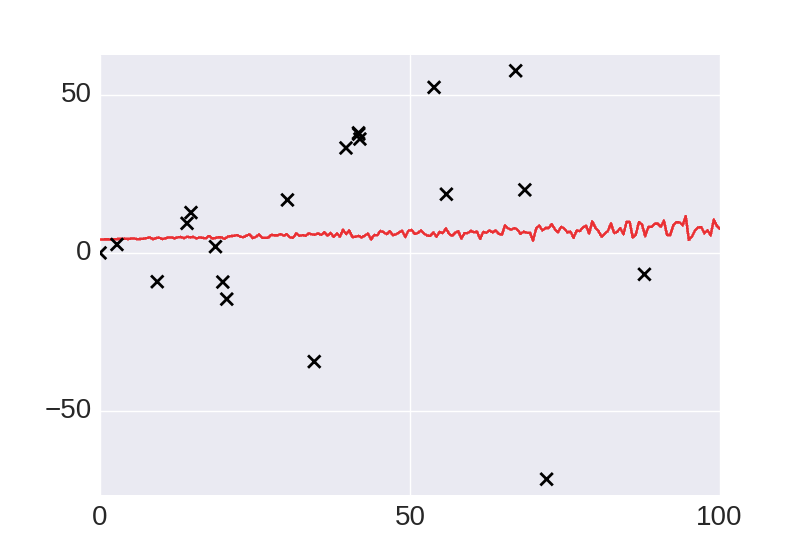
\includegraphics[width=\textwidth]{figs/composition/composition_demo_LIN.png}
        \caption{$\Klin$}
    \end{subfigure}
    ~ %add desired spacing between images, e. g. ~, \quad, \qquad, \hfill etc. 
      %(or a blank line to force the subfigure onto a new line)
    \begin{subfigure}[b]{0.3\textwidth}
        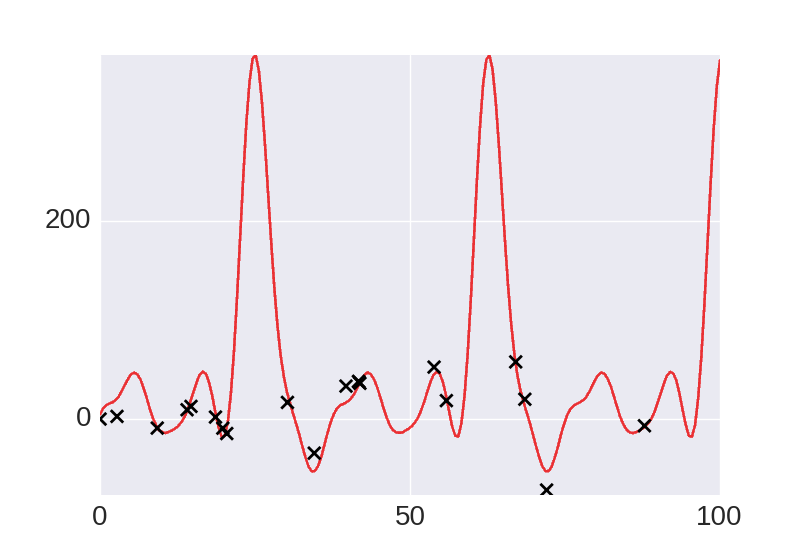
\includegraphics[width=\textwidth]{figs/composition/composition_demo_PER.png}
        \caption{$\Kper$}
    \end{subfigure}
    ~ %add desired spacing between images, e. g. ~, \quad, \qquad, \hfill etc. 
    %(or a blank line to force the subfigure onto a new line)
    \begin{subfigure}[b]{0.3\textwidth}
        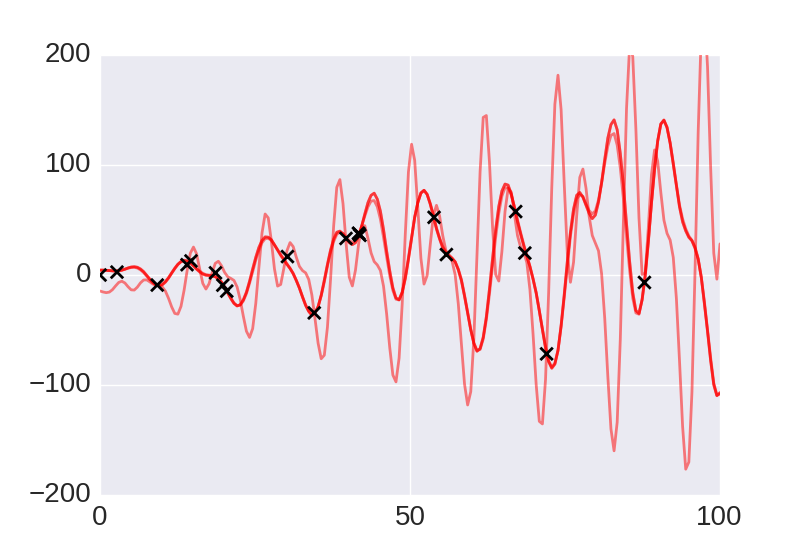
\includegraphics[width=\textwidth]{figs/composition/composition_demo_LINxPER.png}
        \caption{$\Klin \times \Kper$}
    \end{subfigure}

%20.0739791735
%6.31647597198
%37.7184218042
%19.1051376016
